\question[10] Observa los diseños en la figura \ref{fig:sucesion_cuadros01} y responde a las preguntas.

\begin{figure}[H]
    \centering
    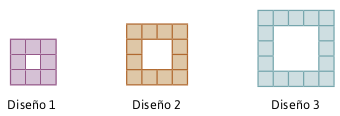
\includegraphics[width=.6\linewidth]{../images/sucesion_cuadros01}
    \caption{}
    \label{fig:sucesion_cuadros01}
\end{figure}

\begin{parts}
    \part ¿Cuántos cuadrados se añaden en cada diseño?

    \begin{solutionbox}{1.5cm}
    \end{solutionbox}

    \part Completa la Tabla \ref{tab:3.5} y luego escribe una regla de recurrencia.

    \begin{solutionbox}{1.5cm}
    \end{solutionbox}

    \begin{table}[H]
        \centering
        \caption{}
        \label{tab:3.5}
        \begin{tabular}{r|c|c|c|c|c|c|c|c|}
            \cline{2-9}
            Posición del diseño & 1                   & 2                     & 3                    & 4                    & 5                    & 6                    & 7                    & 8                    \\ \hline
            Número de cuadrados & \ifprintanswers8\fi & \ifprintanswers12 \fi & \ifprintanswers16\fi & \ifprintanswers20\fi & \ifprintanswers24\fi & \ifprintanswers28\fi & \ifprintanswers32\fi & \ifprintanswers36\fi \\ \cline{2-9}
        \end{tabular}
    \end{table}

\end{parts}

